\chapter{Experiment}
Sensor:\\
Hokuyo UBG 04-LX - 2D scanning laser rangefinder. Measures range\\

Robot arm: \\
Kinova Jaco - can program to move with and record pose

Target object: \\
$0.1 \times 0.1$ m MDF cube, spray painted matte white

1. Collected measurements to model sensor noise for simulation\\
2. Collected measurements of moving cube + measured ground truth cube state - for testing observer with real world conditions

\section{Sensor Noise Characterisation}
	\subsection{Setup}
		physical setup\\
		measurement configurations 
	\subsection{Results}
		data\\
		Histograms (Figure \ref{fig:mean_hist}) - range error approximately normally distributed:
		\begin{figure}
		  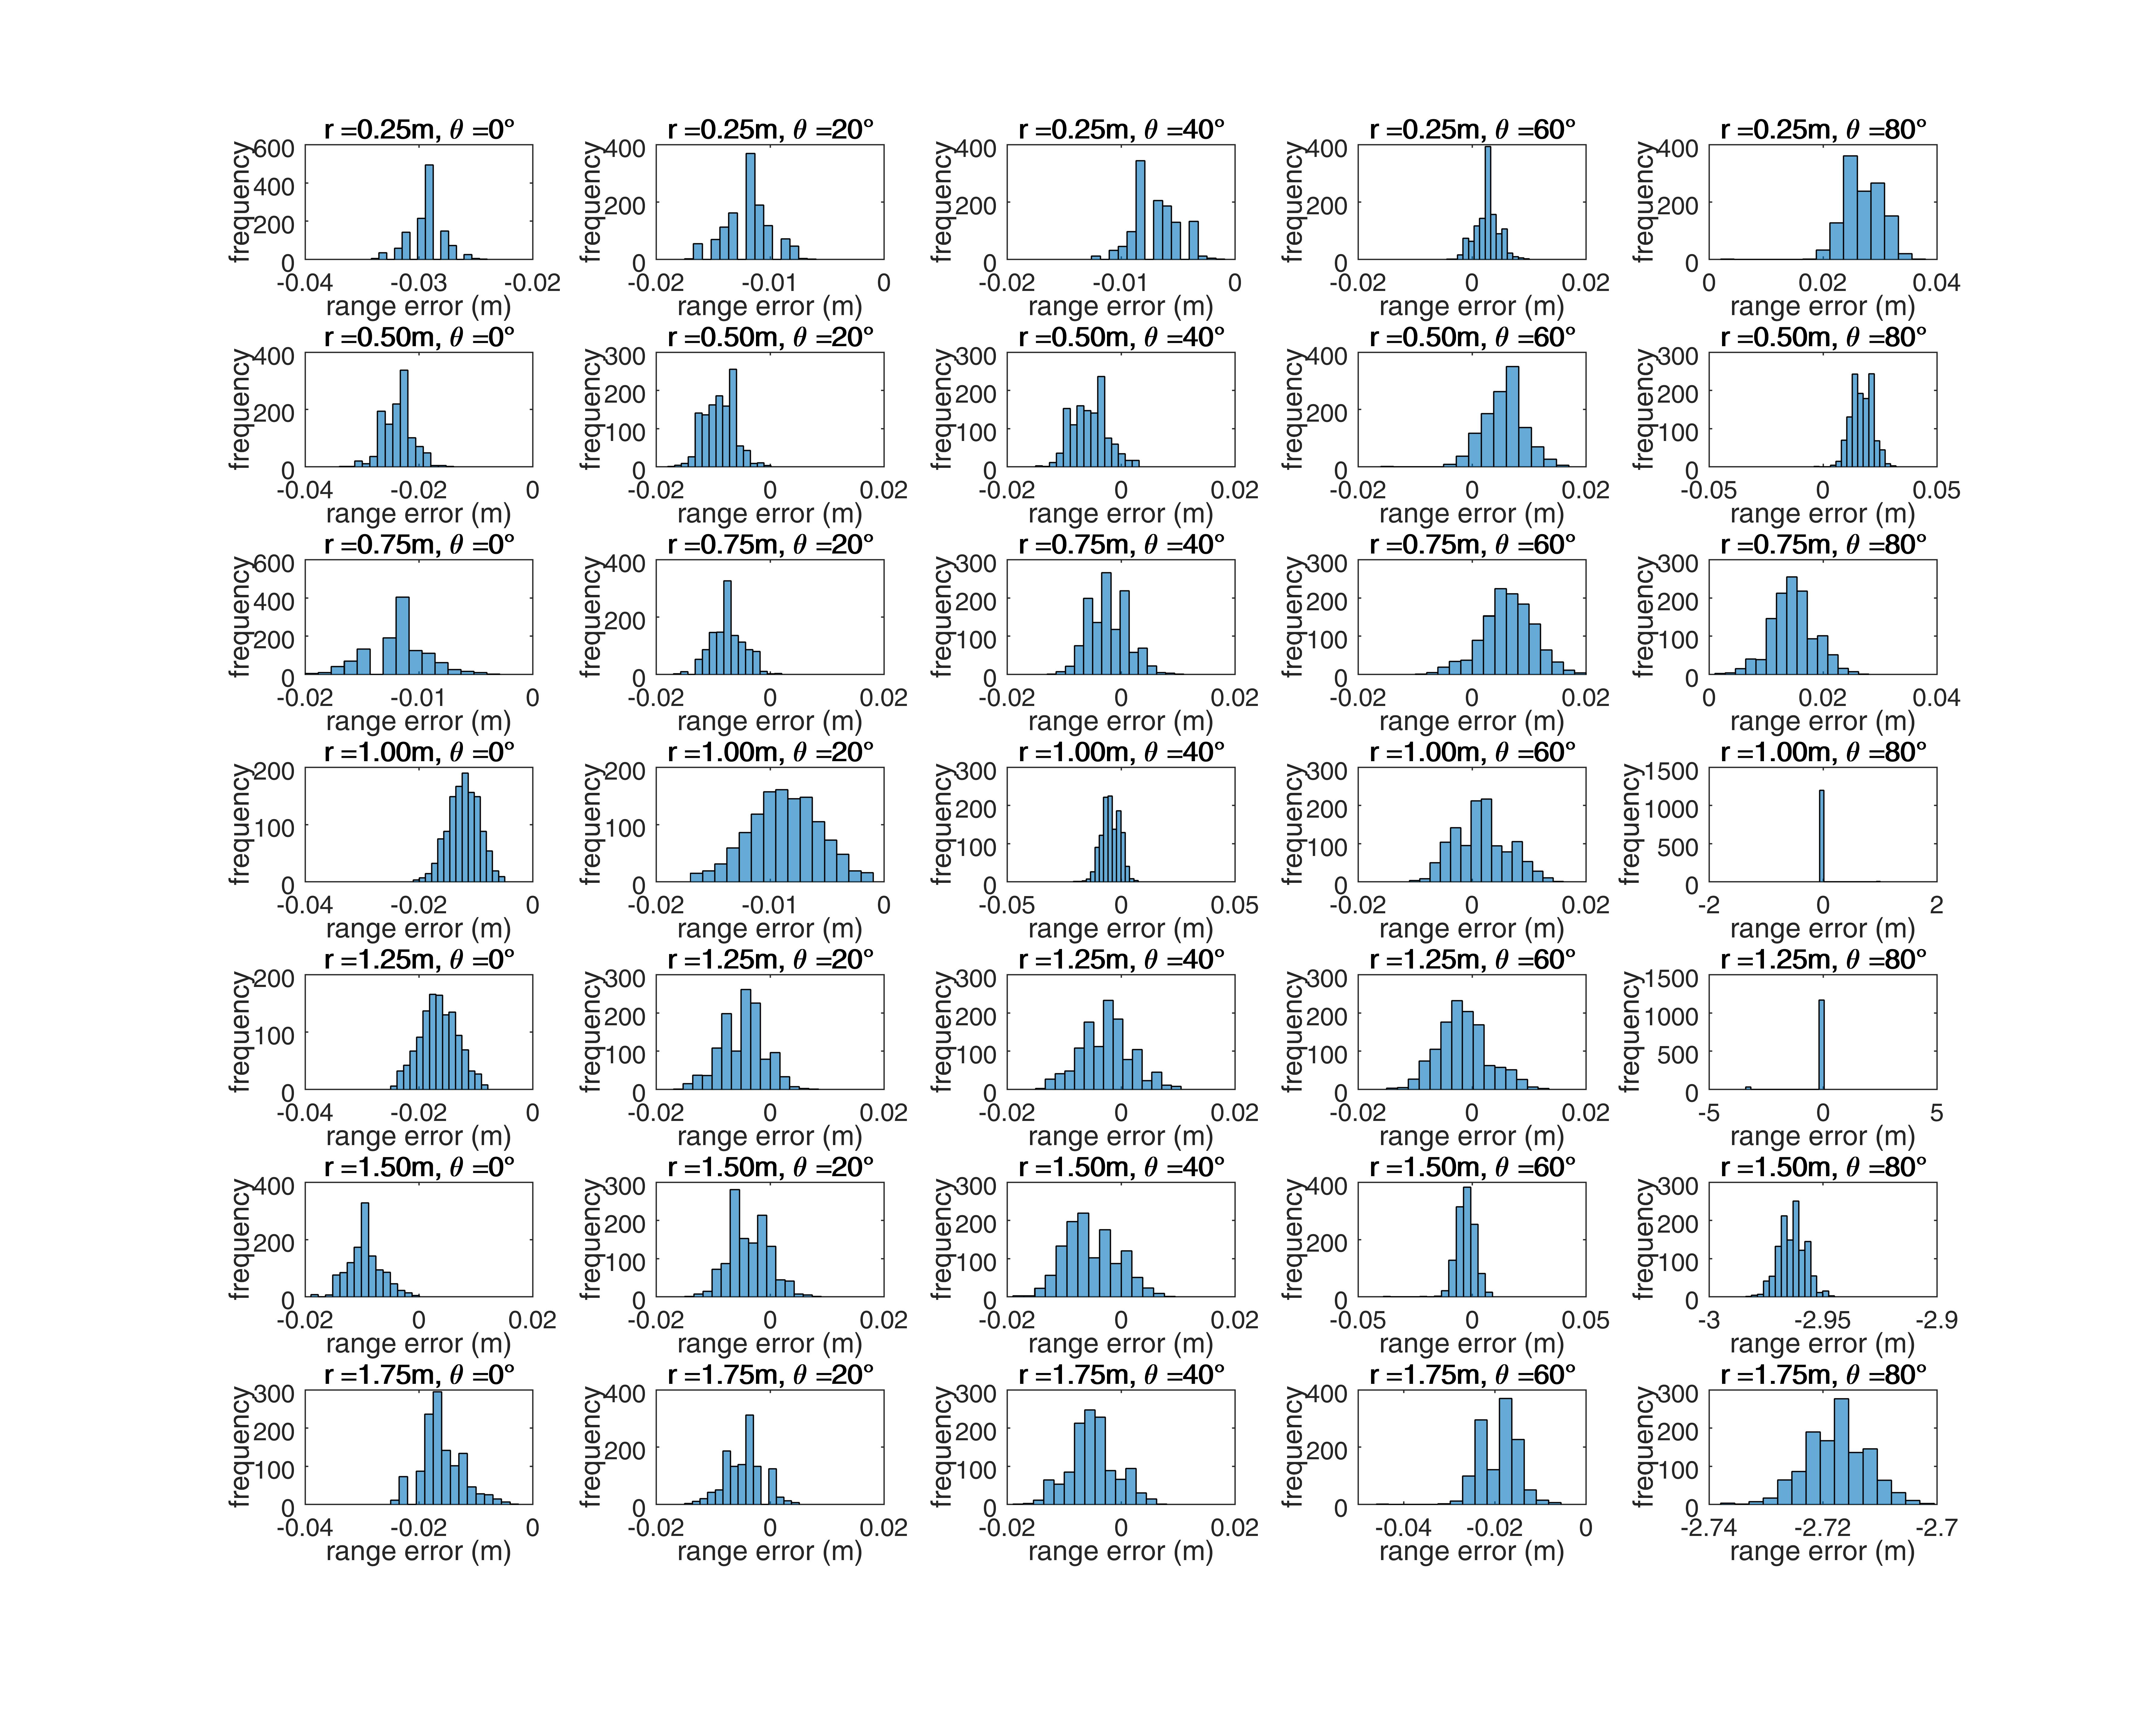
\includegraphics[width=1.25\textwidth,trim = 0mm 0mm 0mm 0mm,clip]{./Figures/range_error_histograms.jpg}
		  \caption{$r_{error}(r,\theta)$ approximately normally distributed}
		  \label{fig:mean_hist}
		\end{figure}
		
		Mean range error - Figure \ref{fig:mean_range_error}
		\begin{figure}
	  		\centering
	  		\subfigure[\label{fig:mean_range_error_outliers}]{
	  		\begin{minipage}[b]{0.45\columnwidth}
    			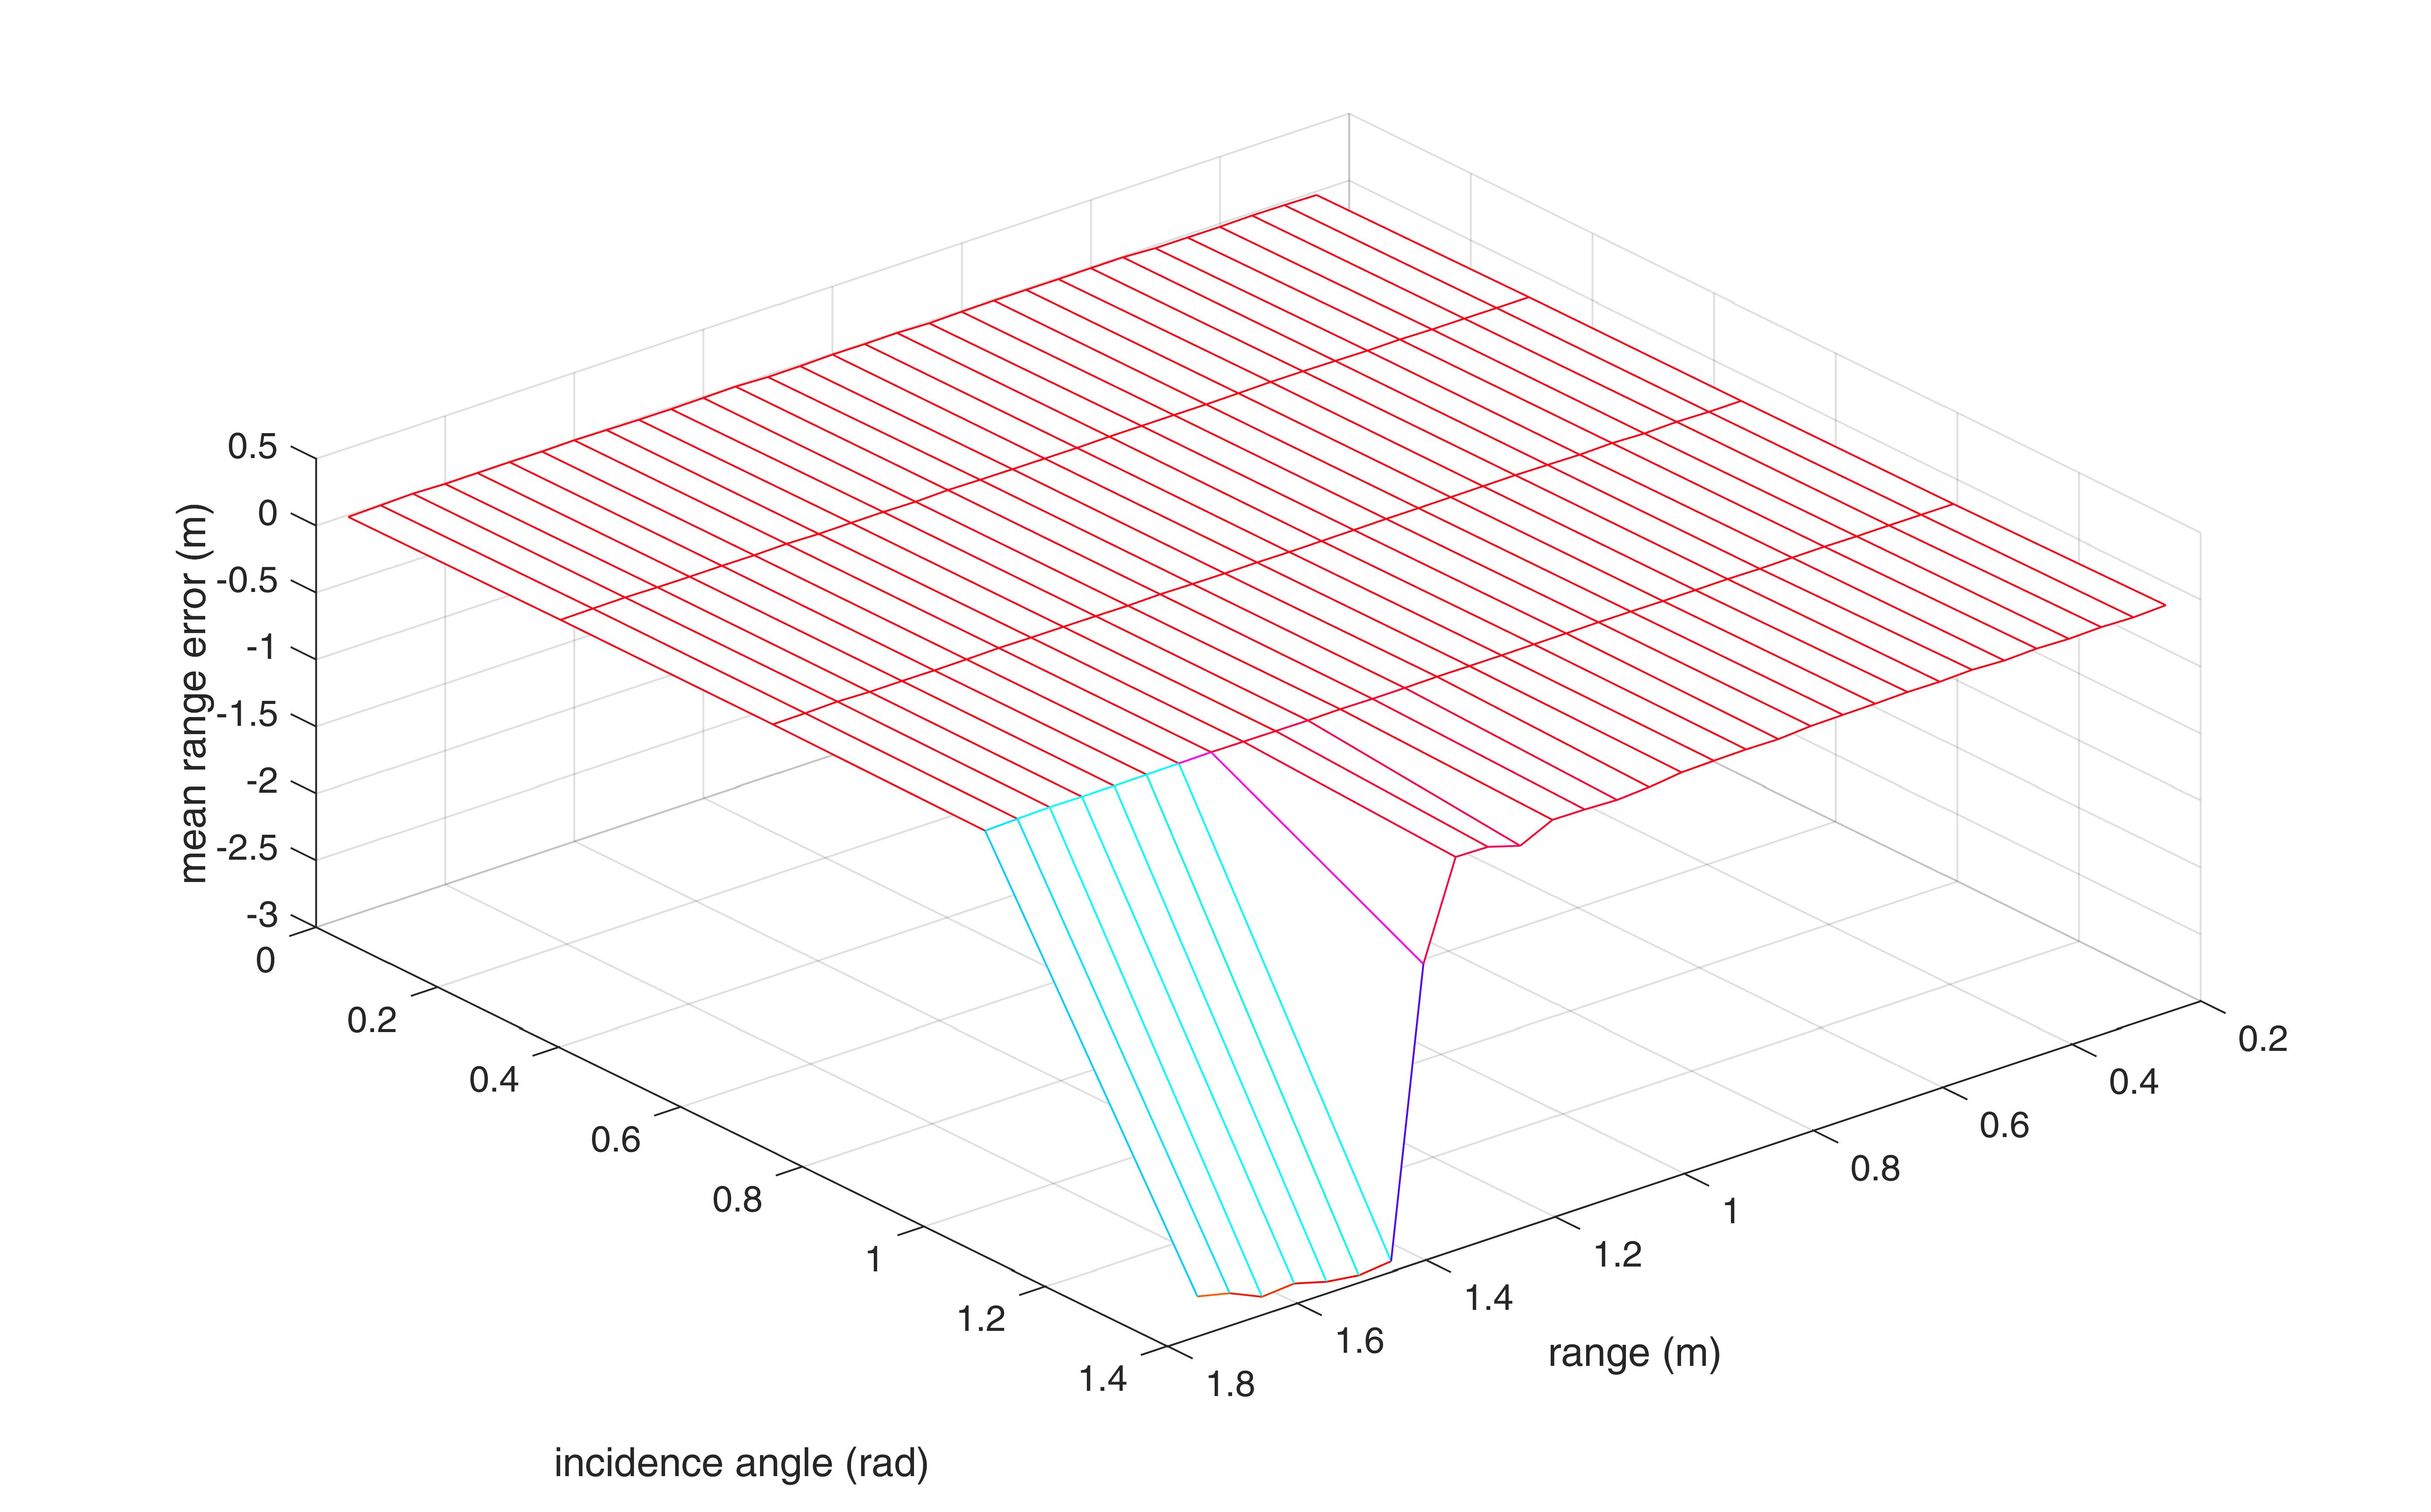
\includegraphics[width=1\textwidth,trim = 0mm 0mm 0mm 0mm,clip]{./Figures/noise_mean_range_error}\vspace*{0ex}
	  		\end{minipage}}
	  		\subfigure[\label{fig:mean_range_error_no_outliers}]{
	  		\begin{minipage}[b]{0.45\columnwidth}
    			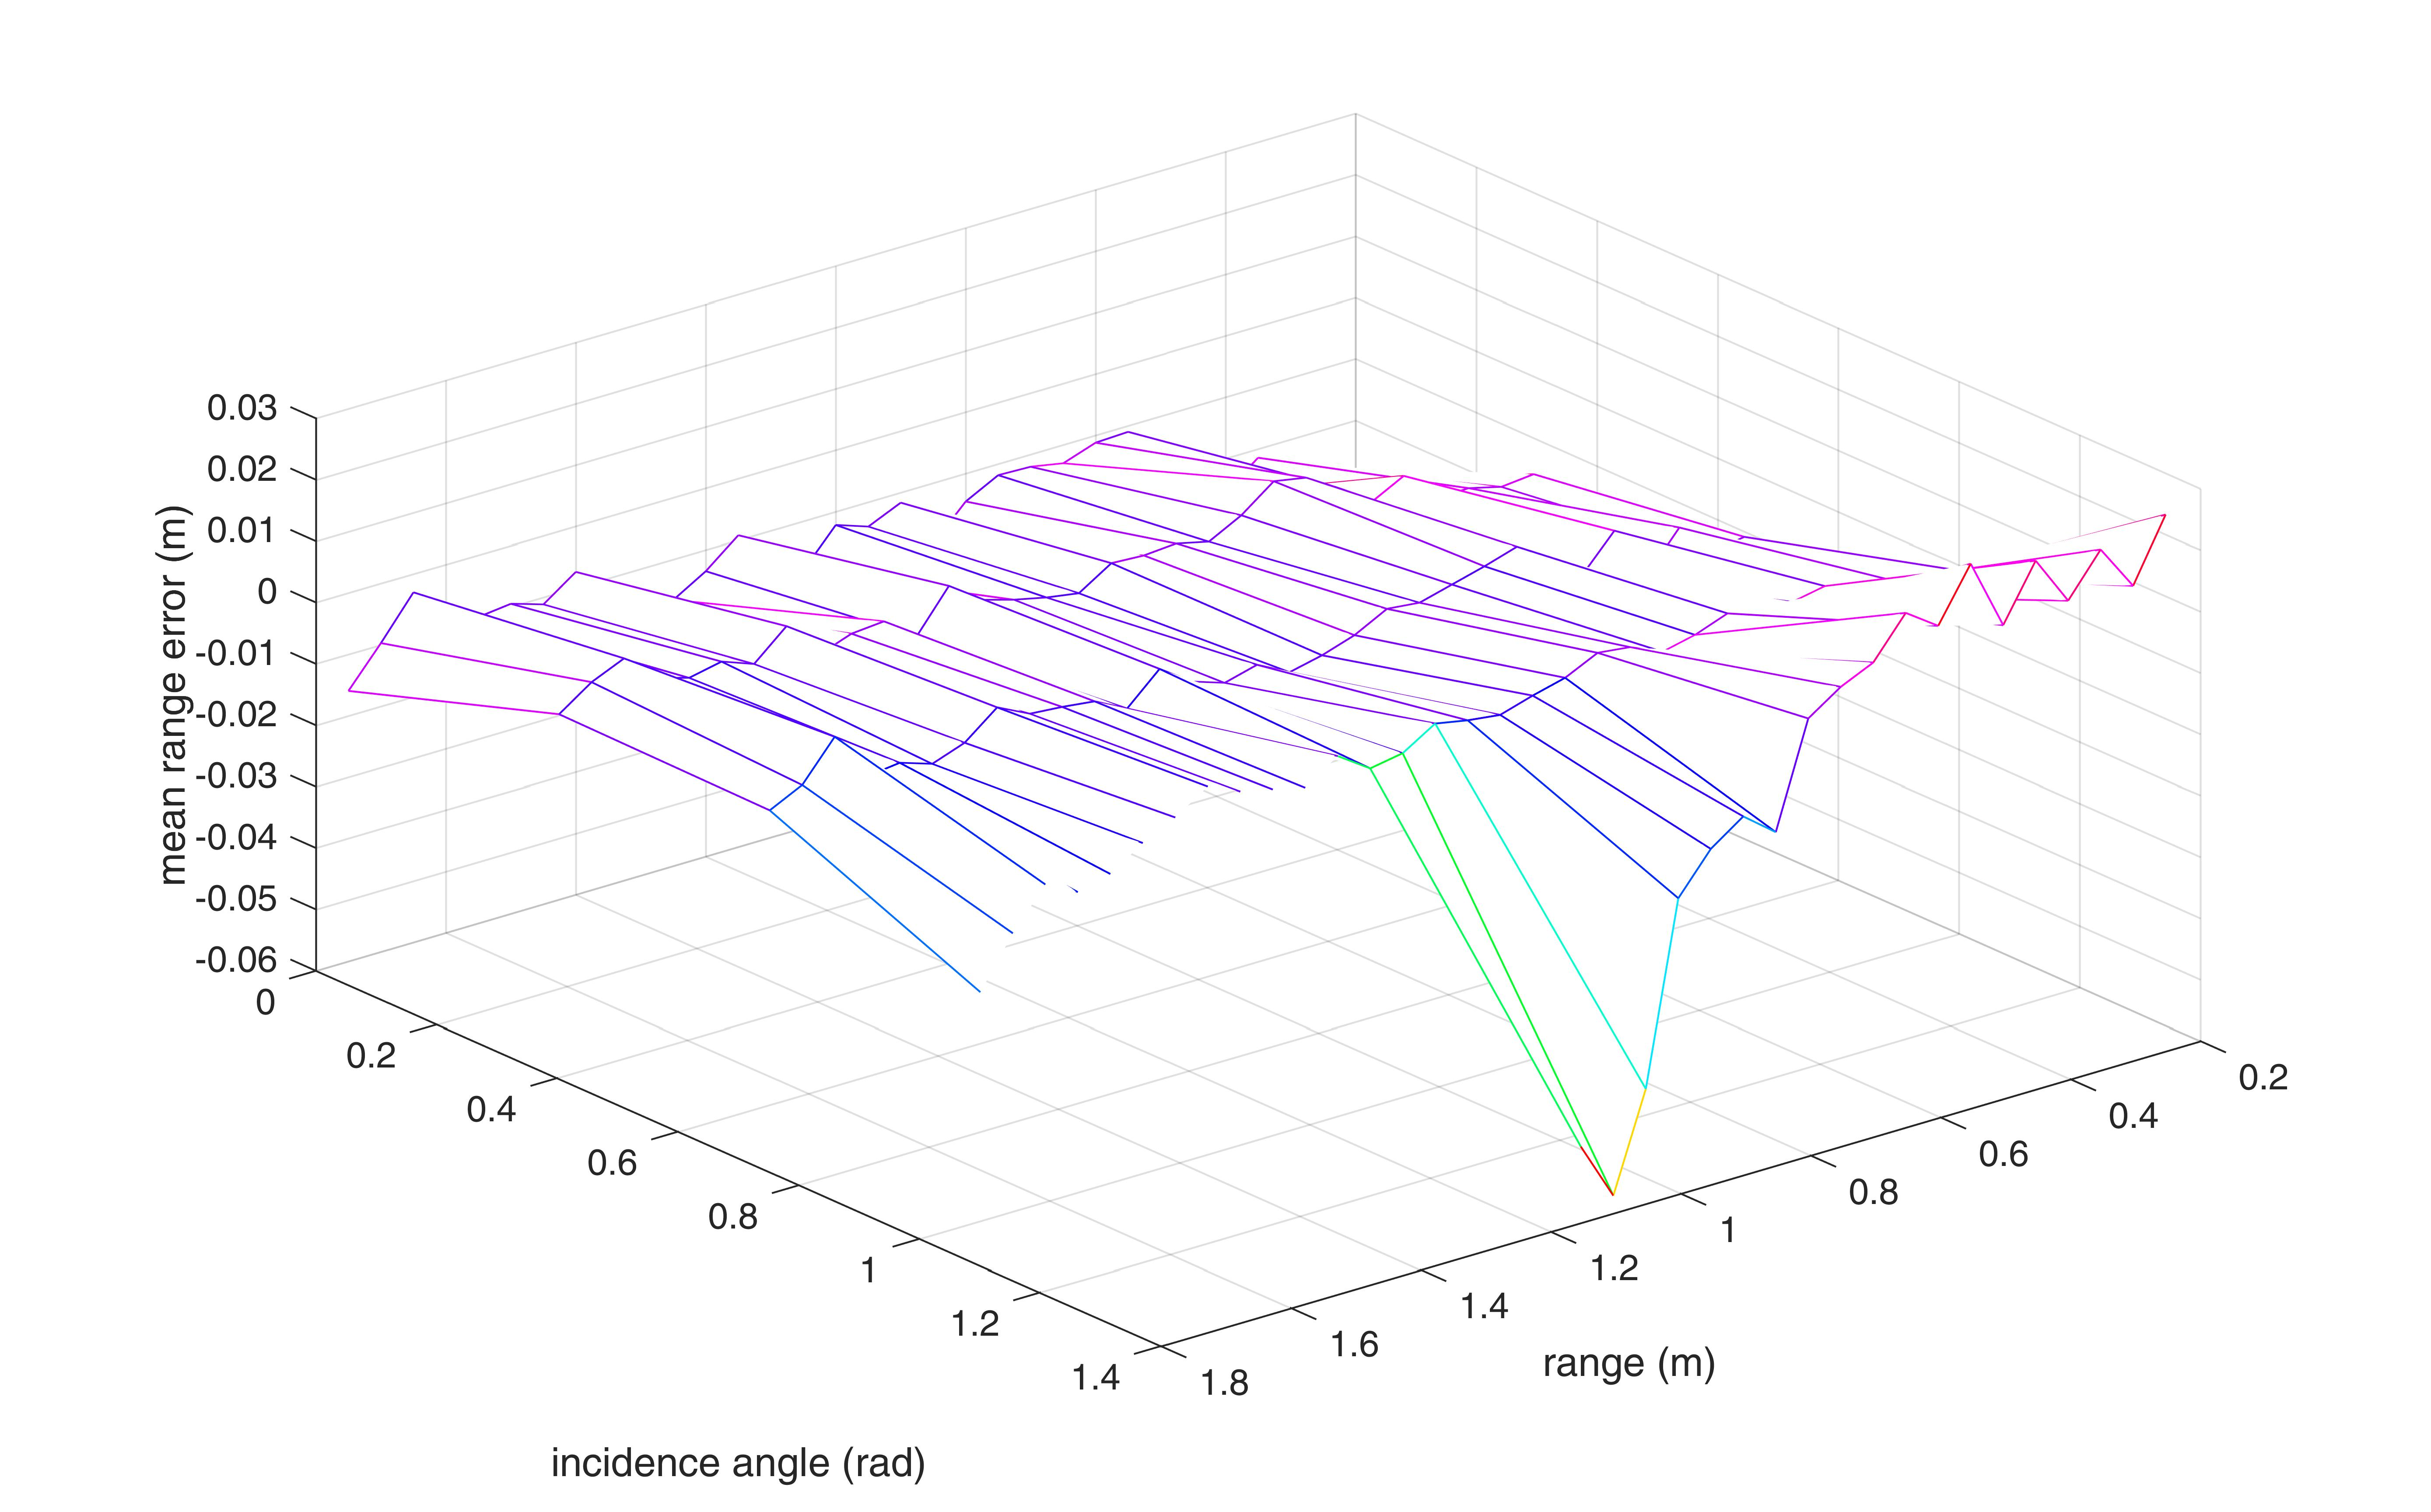
\includegraphics[width=1\textwidth,trim = 0mm 0mm 0mm 0mm,clip]{./Figures/noise_mean_range_error_removed_outliers}\vspace*{0ex}
		 \end{minipage}}
	  		\caption{mean range error vs $(r,\theta)$. (a) large error at high angles and range, (b) overall shape}
	  		\label{fig:mean_range_error}
		\end{figure}
		
		Std dev range error - Figure \ref{fig:stddev_range_error}		
		\begin{figure}
	  		\centering
	  		\subfigure[\label{fig:stddev_range_error_outliers}]{
	  		\begin{minipage}[b]{0.45\columnwidth}
    			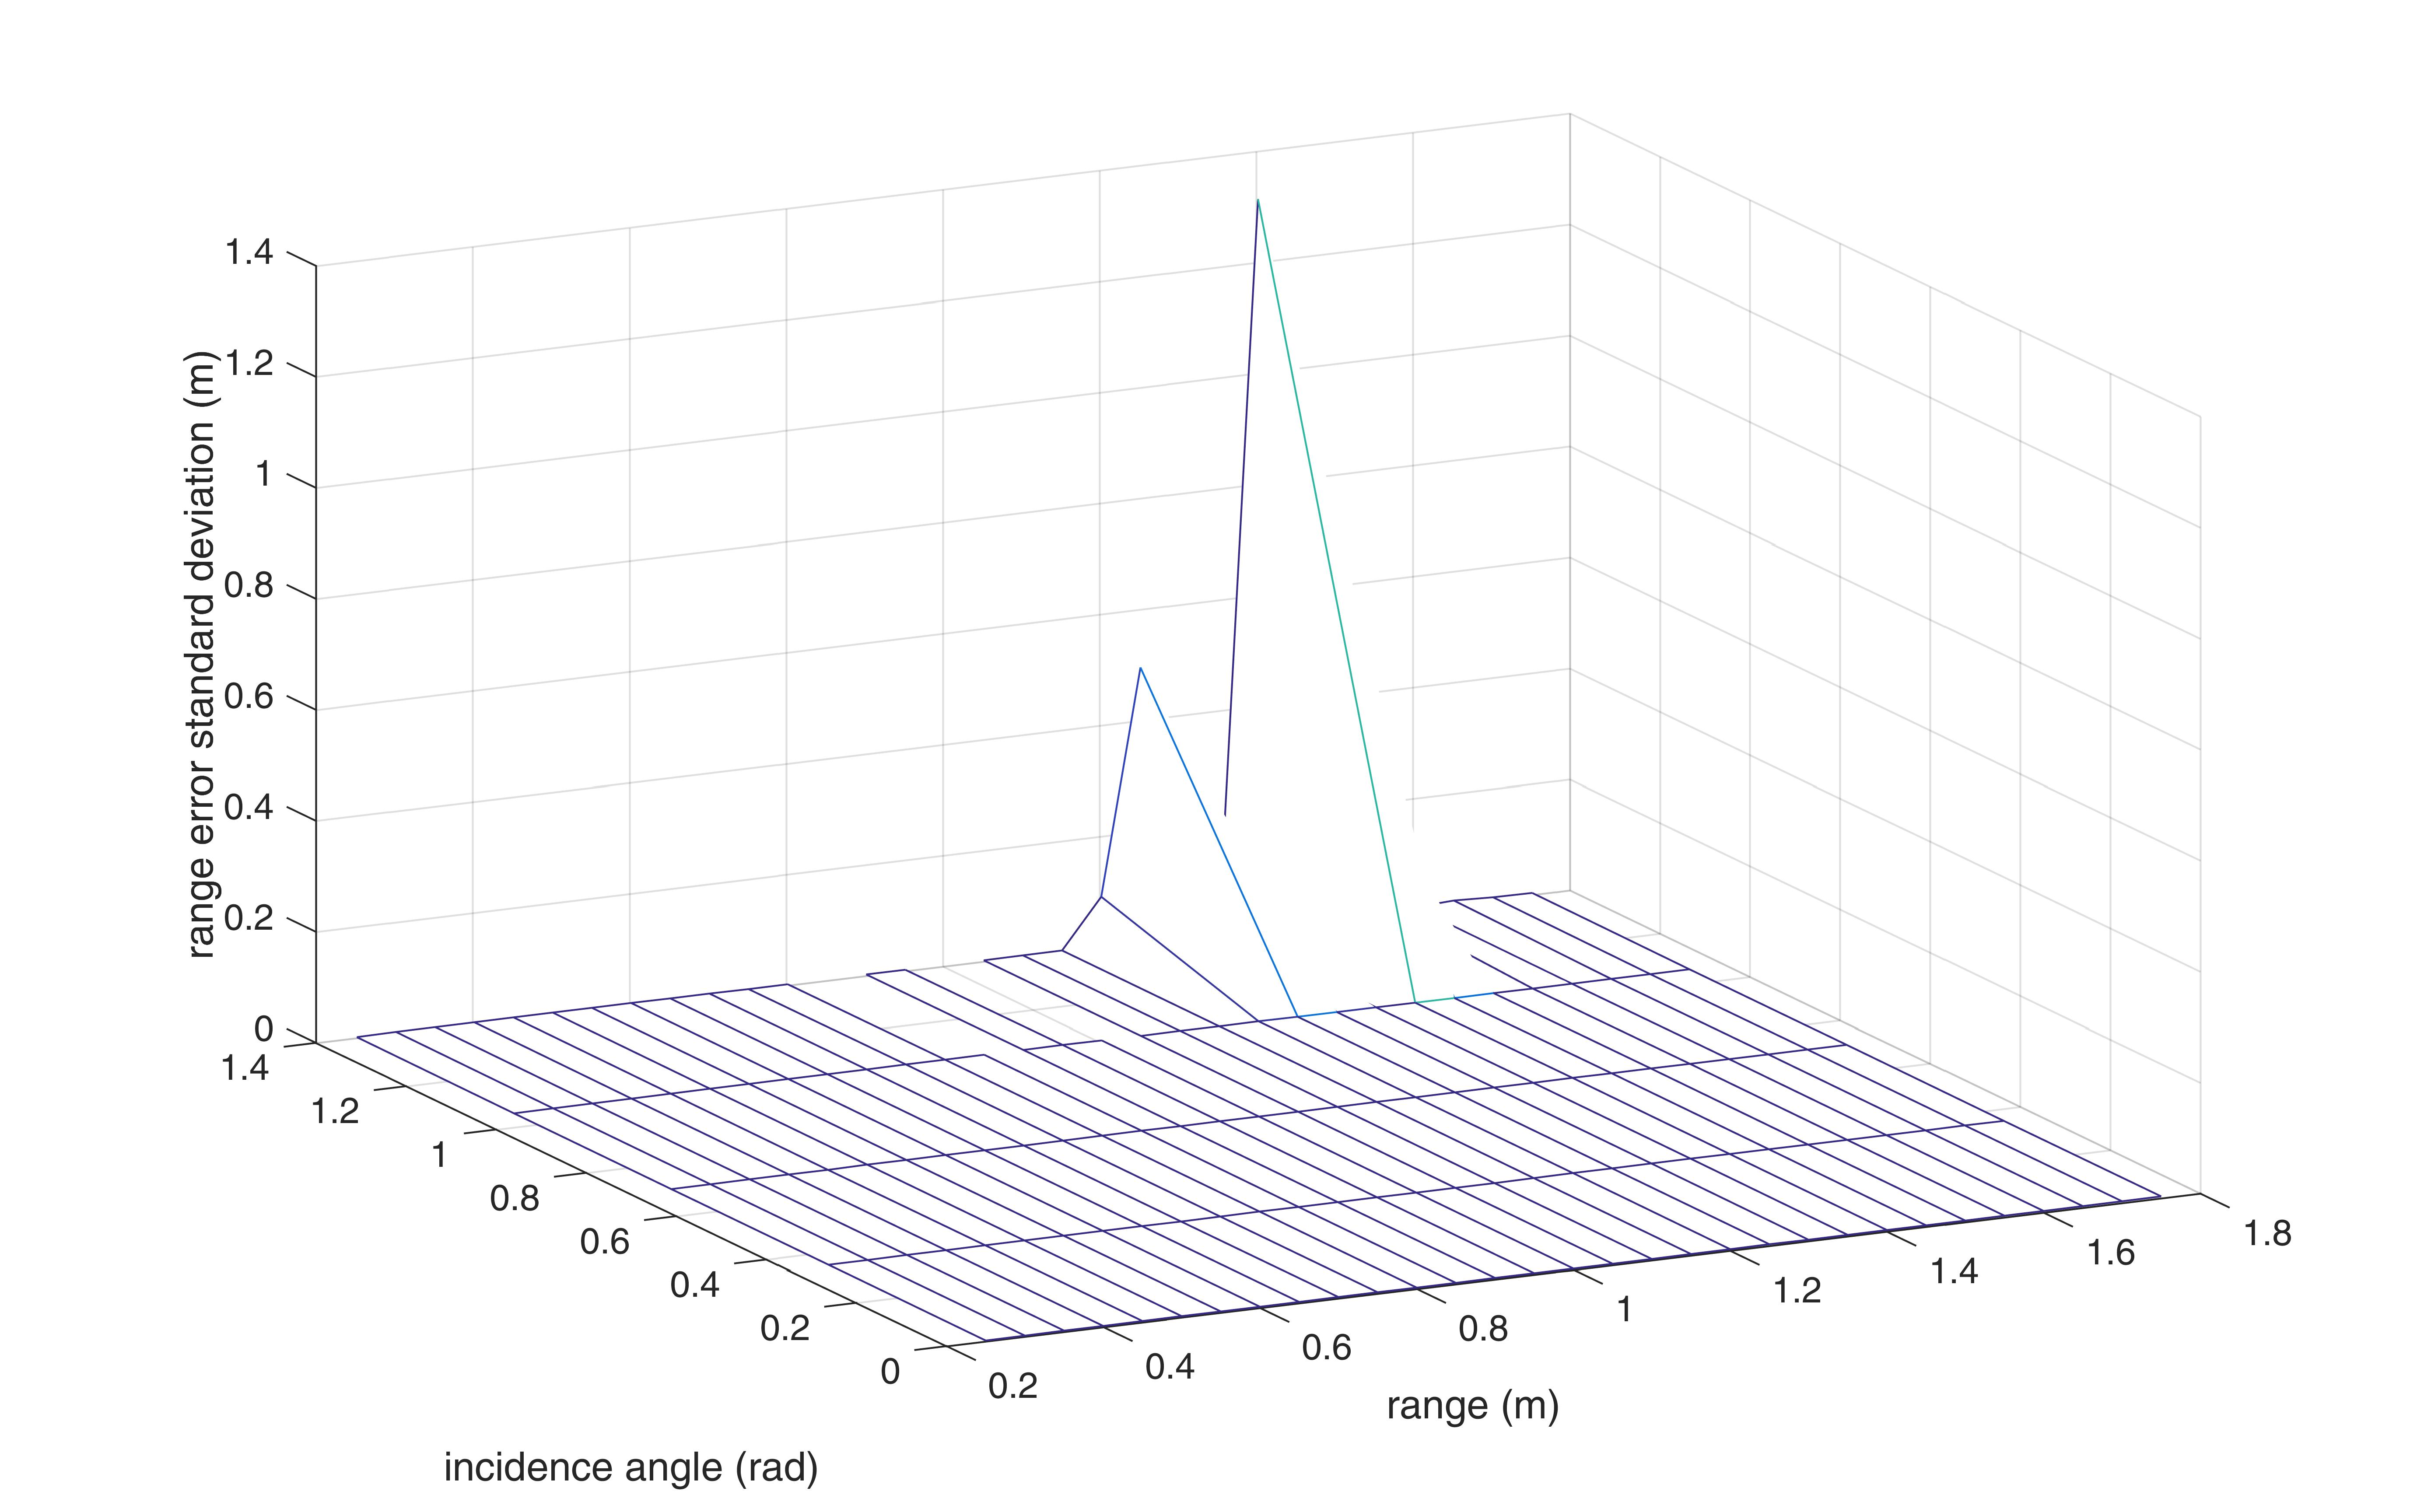
\includegraphics[width=1\textwidth,trim = 0mm 0mm 0mm 0mm,clip]{./Figures/noise_stddev_range_error}\vspace*{0ex}
	  		\end{minipage}}
	  		\subfigure[\label{fig:stddev_range_error_no_outliers}]{
	  		\begin{minipage}[b]{0.45\columnwidth}
    			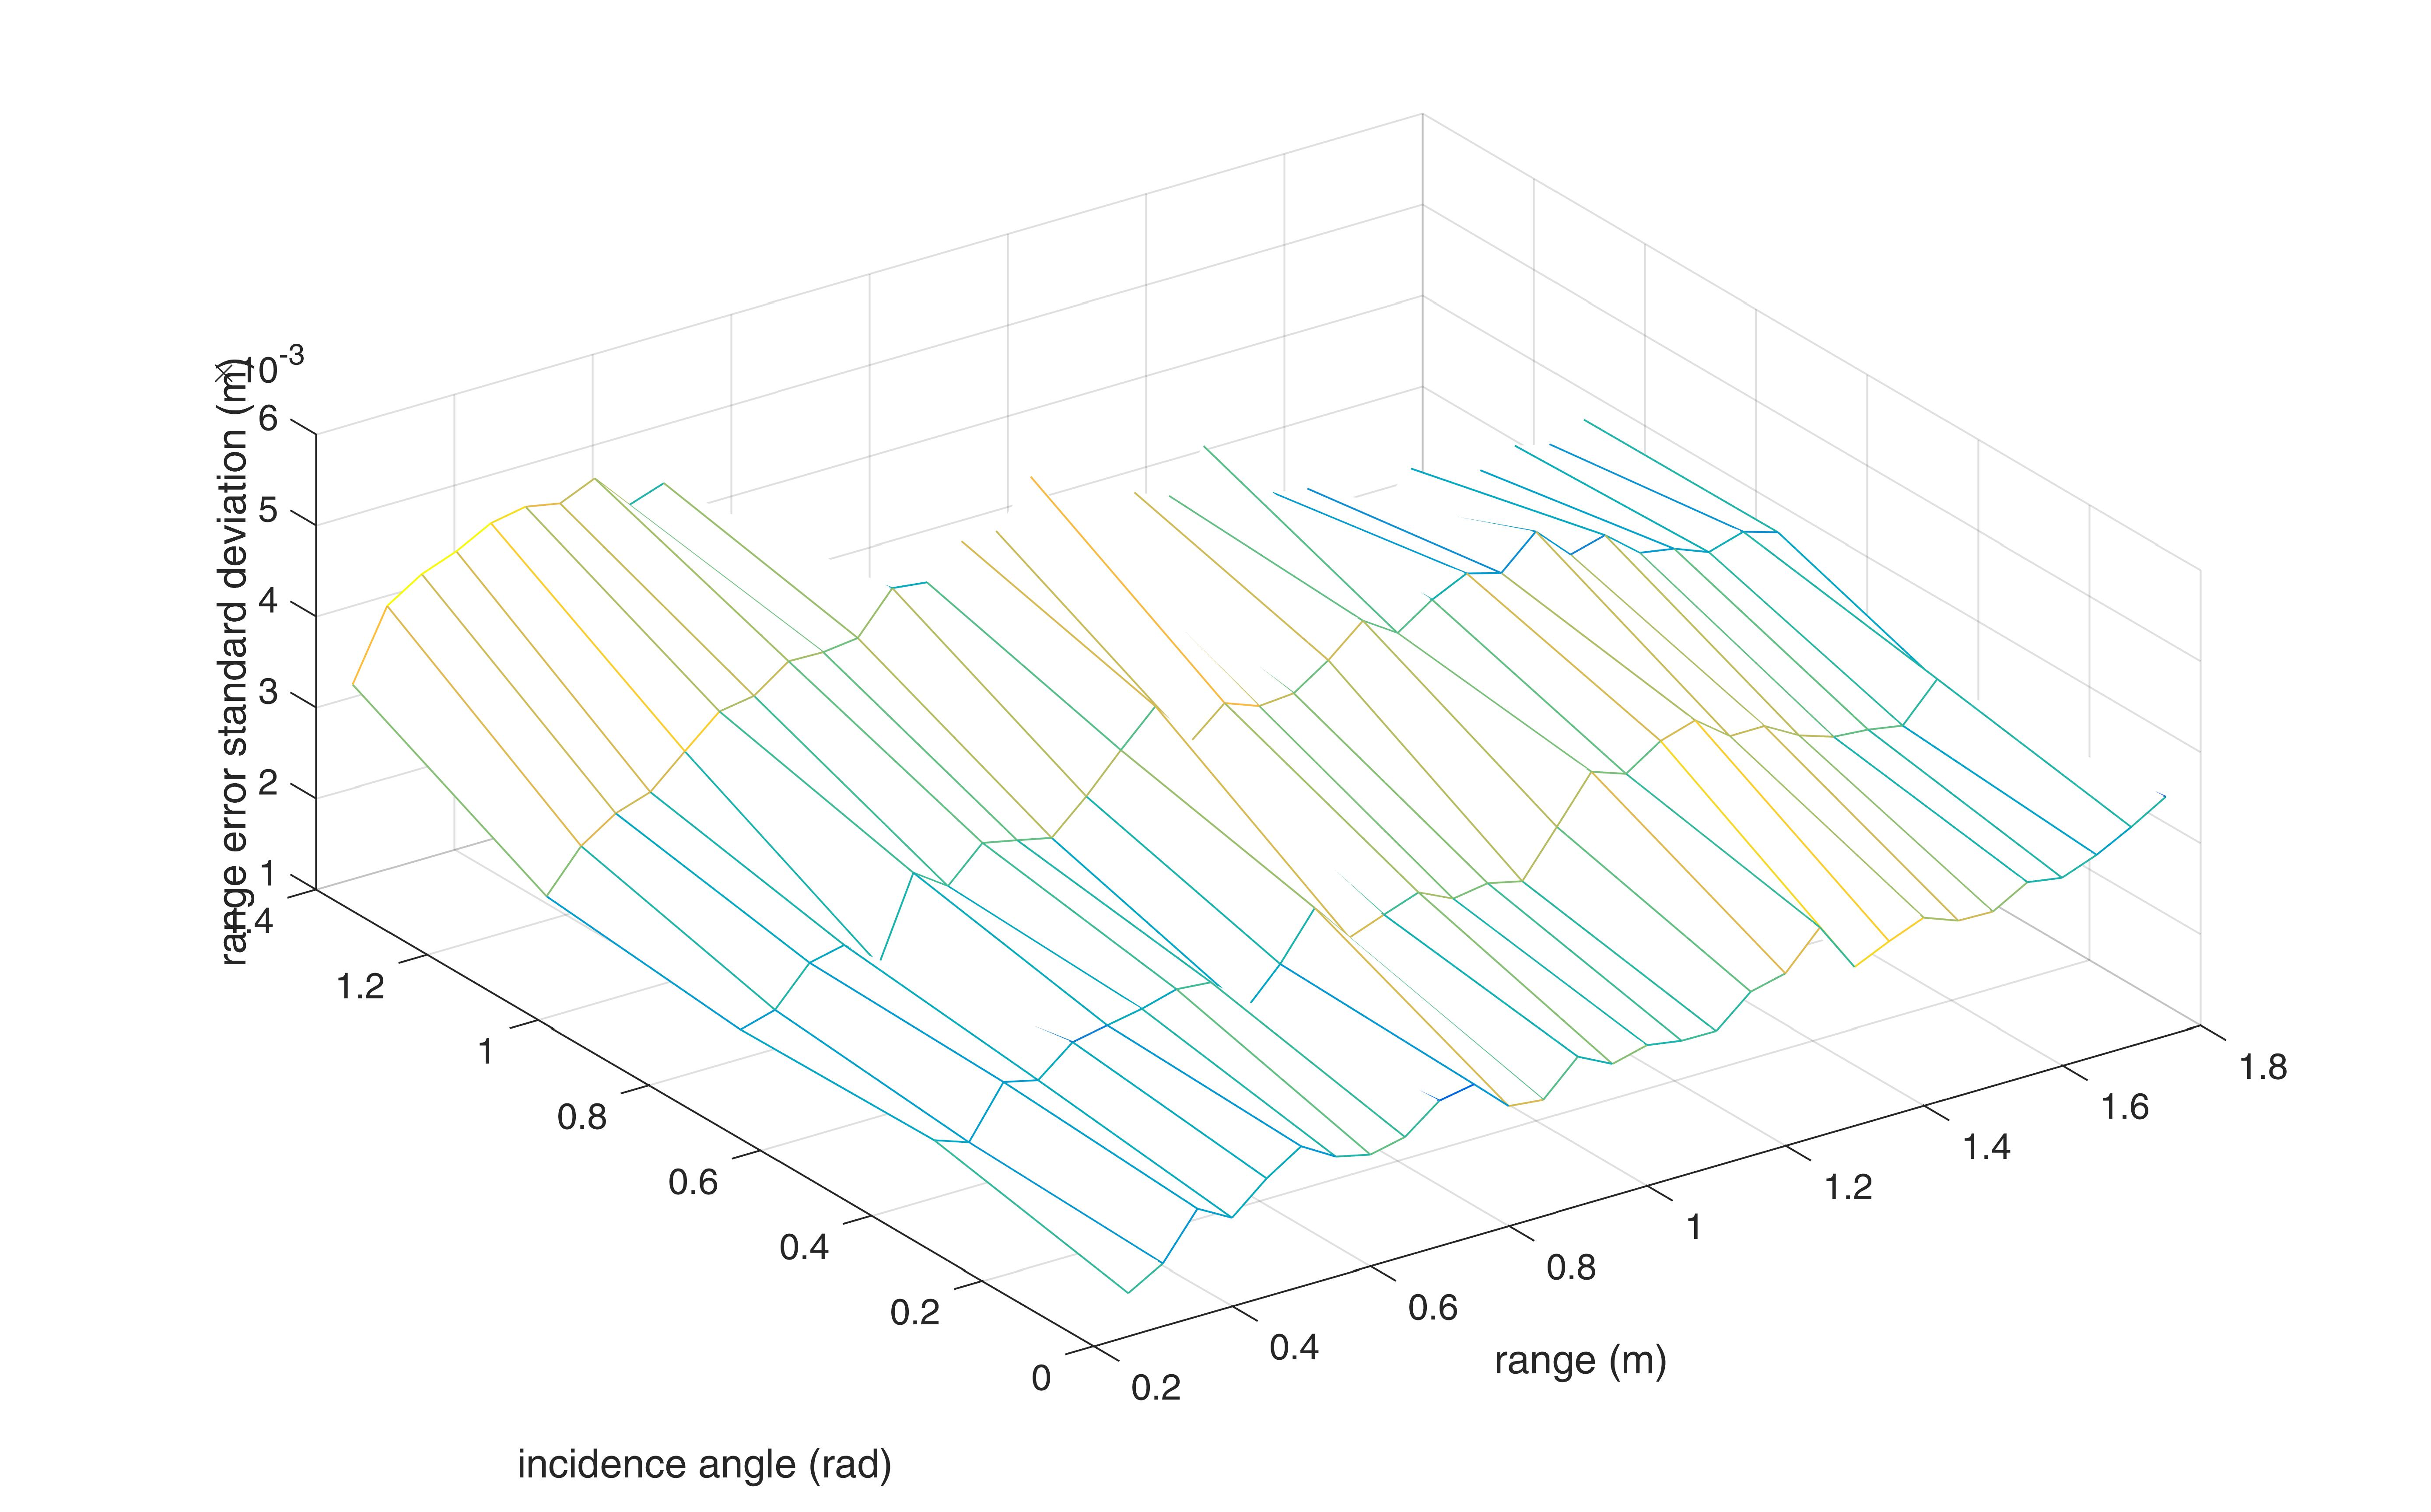
\includegraphics[width=1\textwidth,trim = 0mm 0mm 0mm 0mm,clip]{./Figures/noise_stddev_range_error_removed_outliers}\vspace*{0ex}
	 		 \end{minipage}}
	  		\caption{range error $\sigma$ vs $(r,\theta)$. (a) outliers/large std dev at high angles and range, (b) overall shape}
	  		\label{fig:stddev_range_error}
		\end{figure}
		
		Fitted 4th degree (in $x$ and $y$) polynomials to data points - Figure \ref{fig:surface_range_error}
		\begin{figure}
	  		\centering
	  		\subfigure[\label{fig:surface_mean_range}]{
	  		\begin{minipage}[b]{0.45\columnwidth}
    			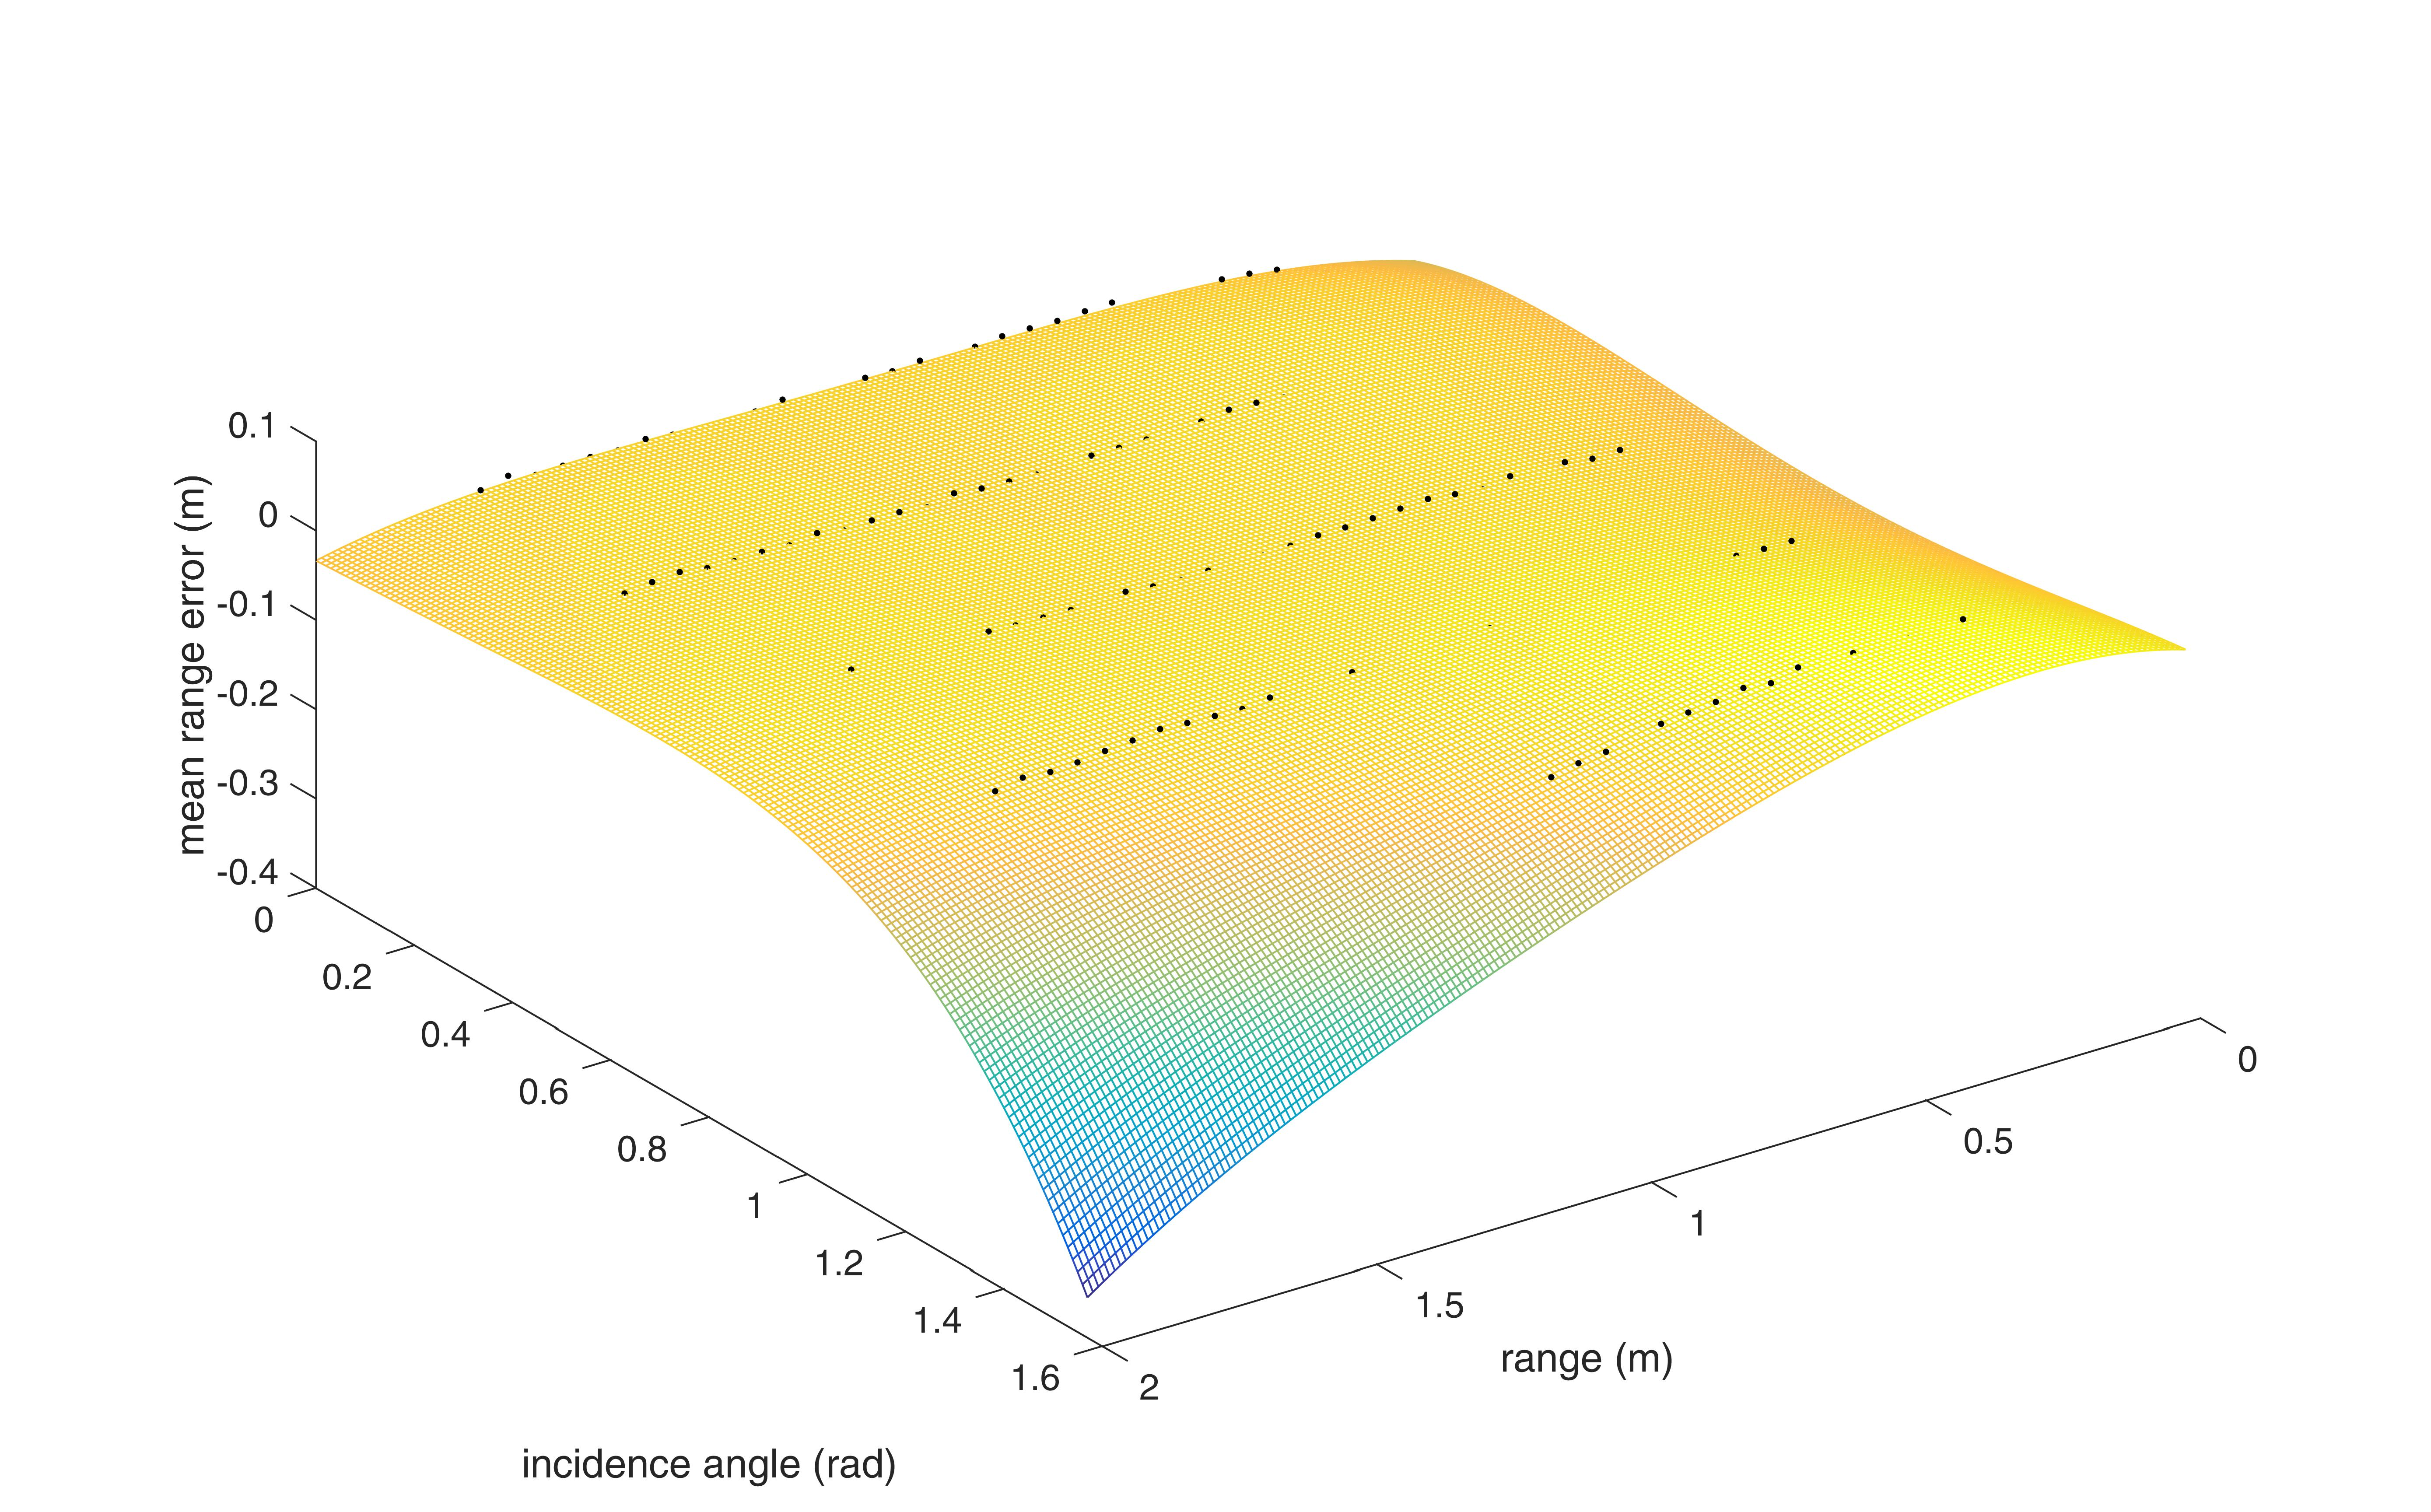
\includegraphics[width=1\textwidth,trim = 0mm 0mm 0mm 0mm,clip]{./Figures/surface_mean_range_error}\vspace*{0ex}
	  		\end{minipage}}
	  		\subfigure[\label{fig:surface_stddev_range}]{
	  		\begin{minipage}[b]{0.45\columnwidth}
    			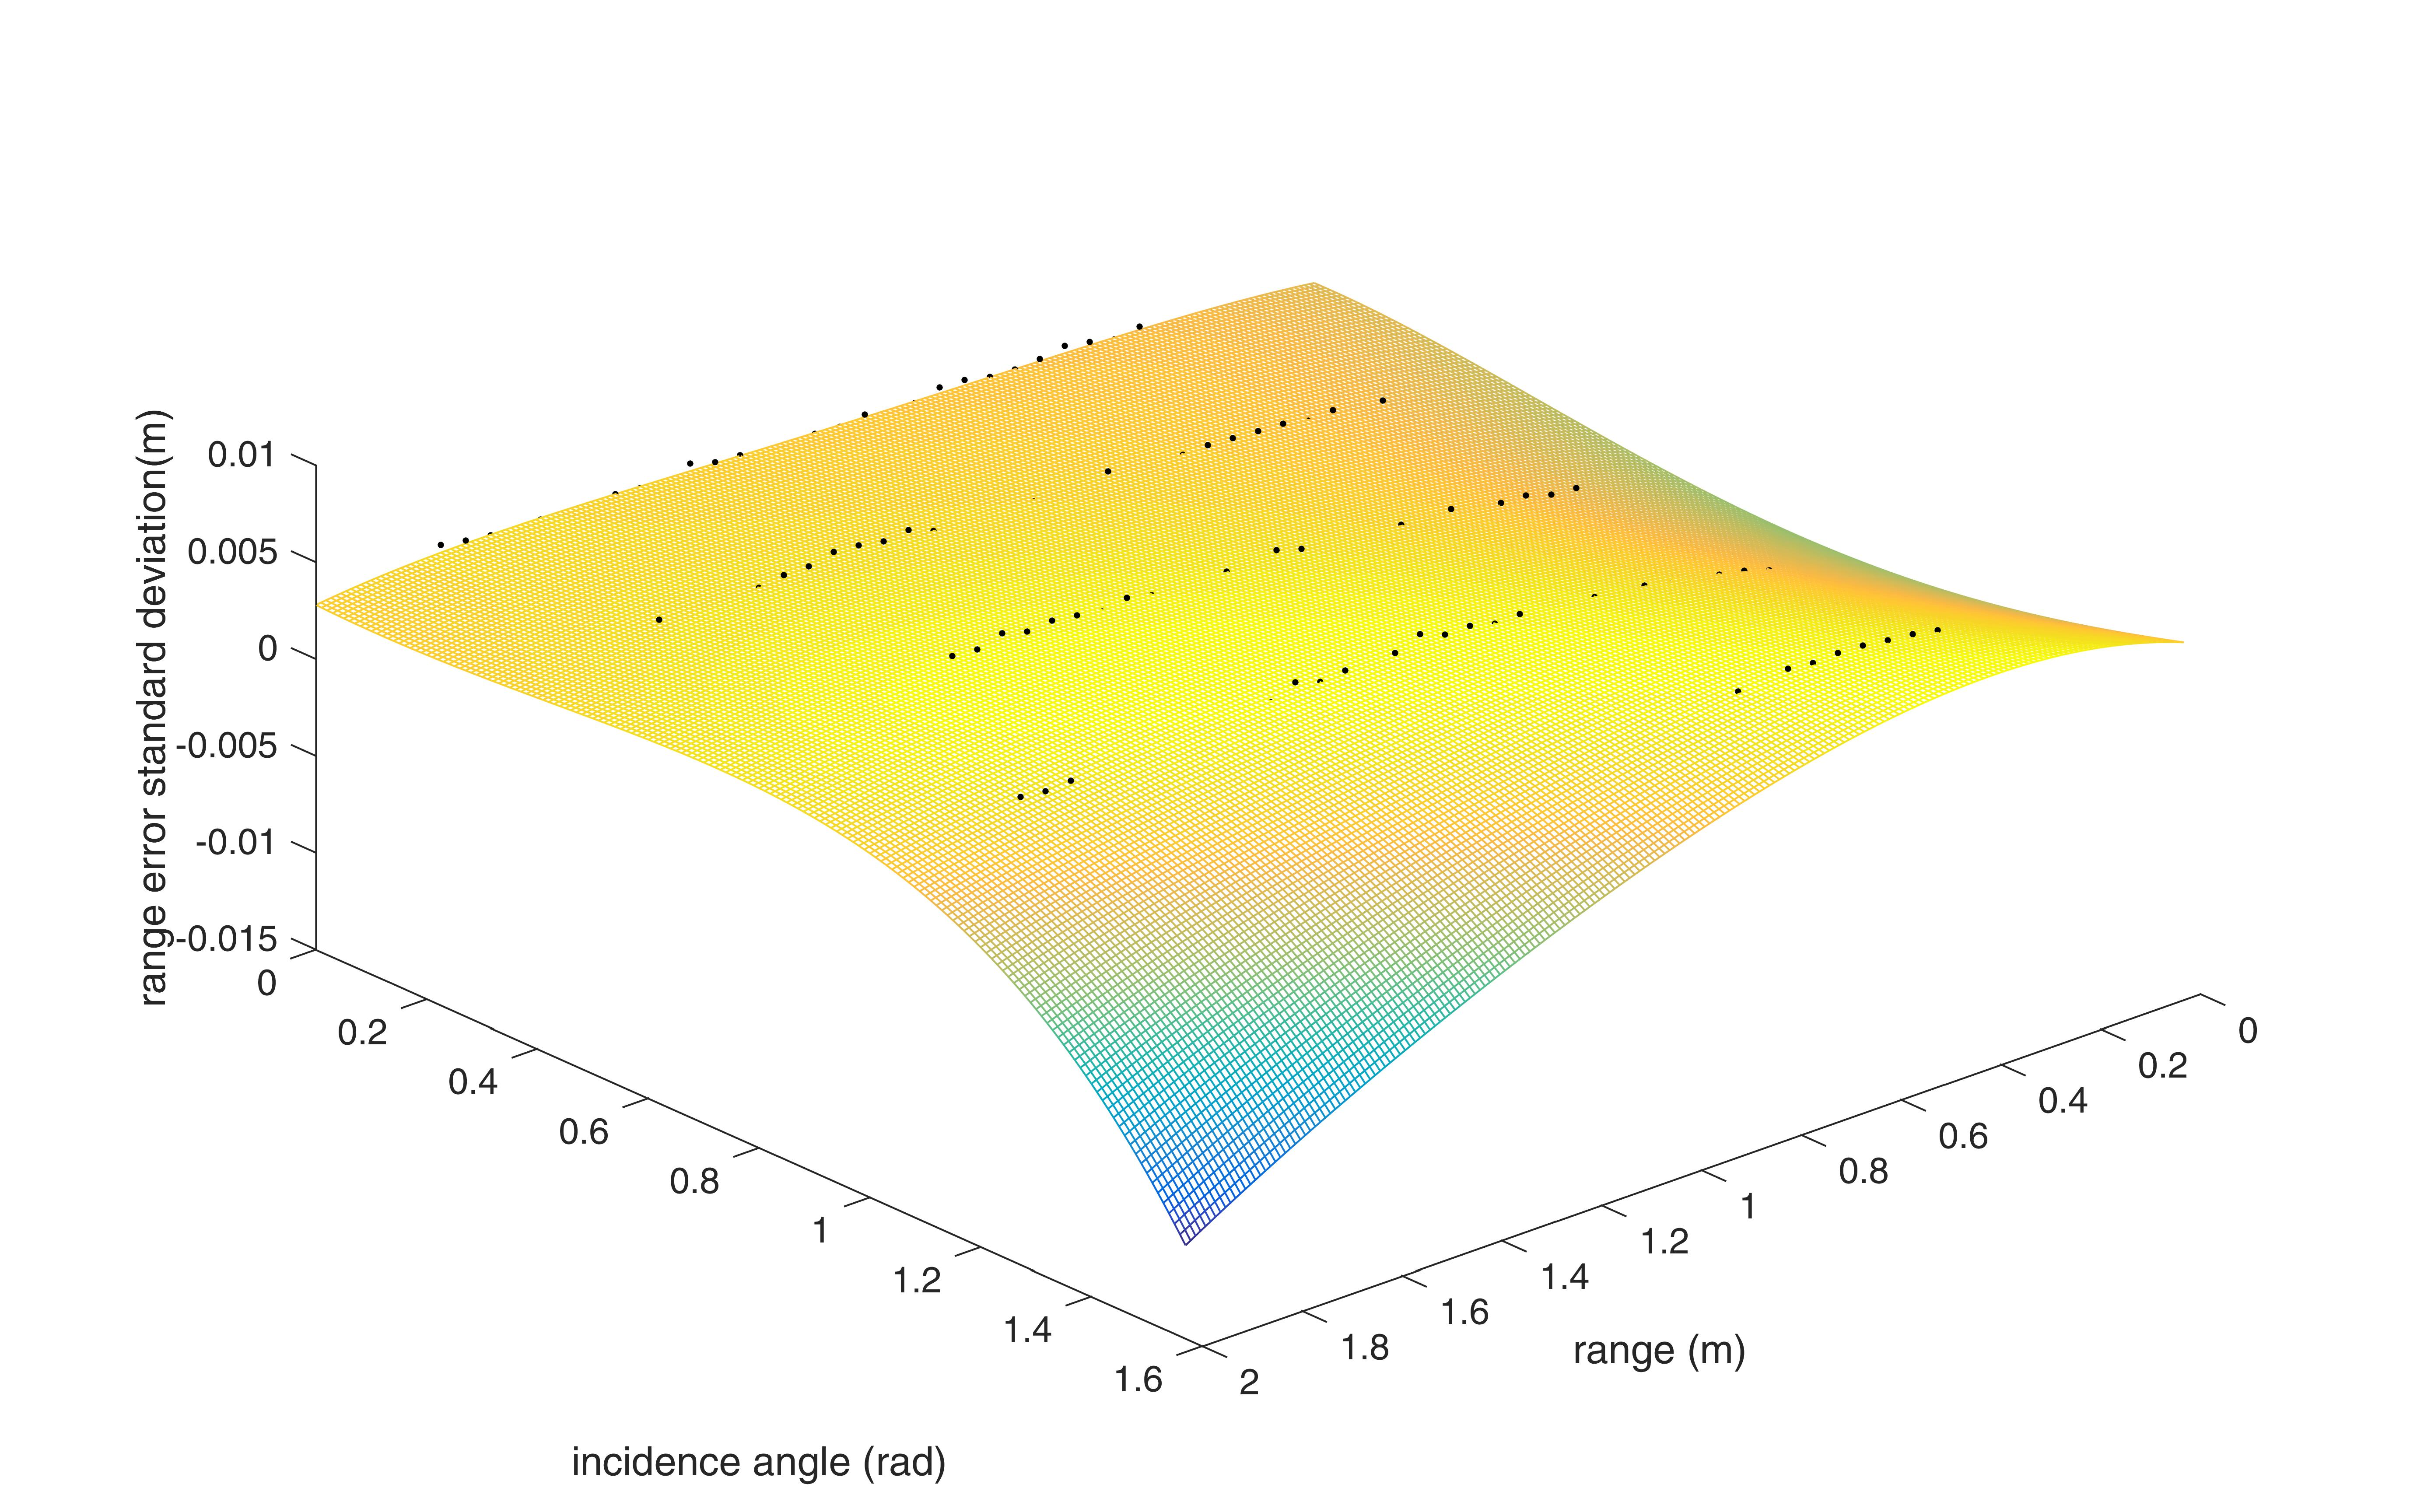
\includegraphics[width=1\textwidth,trim = 0mm 0mm 0mm 0mm,clip]{./Figures/surface_stddev_range_error}\vspace*{0ex}
		 \end{minipage}}
	  		\caption{polynomials fitted to range error mean \& standard deviation data points to model noise}
	  		\label{fig:surface_range_error}
		\end{figure}
		
		\begin{equation}
			r_{error} = r + \mathcal{N}(\mu,\sigma)
		\end{equation}	
		noise model
		\begin{equation}	
			 	\mu = a_{00} + a_{10}r + a_{01}\theta + a_{20}r^2 + a_{11}r\theta + a_{02}\theta^2
			 	      + a_{30}r^3 + a_{21}r^2\theta + a_{12}r\theta^2 + a_{03}\theta^3 + a_{40}r^4 + a_{31}r^3\theta + {22}r^2\theta^2 + a_{13}r\theta^3 + a_{04}\theta^4 	
		\end{equation}
		\begin{equation}
			\sigma = 
		\end{equation}
		
		*random walk surface noise model here too?\\
		surface properties (or sensor processing) error on mean range across surface, looks sinusoidal, peaks = 5mm deep \& 50mm wide approximately - seems to be independent of range and angle\\
		random walk model

\section{Testing Data Collection}
	\subsection{Setup}
		physical setup\\
		configurations/motions\\
		arm forward kinematics $\rightarrow$ cube pose\\
		estimate sensor angle with horizontal with wall calibration data		
		
	\subsection{Results}
		observer performance

